\documentclass{beamer}
\usetheme{default}
%\usetheme{JuanLesPins}
\usepackage{listings}
\usepackage{times}

%\usepackage{xkeyval}
\usefonttheme{structurebold}

\usepackage[english]{babel}
%\usepackage{pgf,pgfarrows,pgfnodes,pgfautomata,pgfheaps,graphics}\usepackage{pgflibraryshapes}
\usepackage{graphics}
\usepackage{epsfig}
\usepackage{amsmath,amssymb}
\usepackage[latin1]{inputenc}


%%%%%%%%%%%%%%%%%%%%%%%CARDIS 06%%%%%%%%%%%%%%%%%%%%%55
\usepackage{tikz}
\usepackage{pgflibraryshapes}
\usepackage{listings}
\lstset{escapeinside={(*@}{@*)}}
\lstset{commentstyle=\color{blue!50!black}\textit,tabsize=2,keywordstyle=\color{green!50!black}}
\lstset{backgroundcolor=\color{lightgray!50}}
%\lstset{frame=trbl,frameround=DDDD}
\lstset{numbers=left, numberstyle=\footnotesize}
\usepackage{multirow}
\newcommand{\benchname}[1]{\texttt{#1}}
\setbeamercovered{dynamic}
\beamertemplatenavigationsymbolsempty

%\AtBeginSection[]{\frame{\frametitle{Outline}\tableofcontents[current]}}

\begin{document}
\title{Bytecode Verification and Specification}
\author{Mariela Pavlova}

\maketitle

\newcommand{\program}{\mbox{\rm\texttt{P}}}%\xspace}

\newcommand{\subst}[2]{[ #1 \leftarrow #2]}
\newcommand{\requires}{\texttt{requires}}
\newcommand{\ensures}{\texttt{ensures}}
\newcommand{\annotation}{BML}
\newcommand{\exsures}[1]{ \texttt{exsures} (#1)}
\newcommand{\invariant}{ \texttt{invariant}}
\newcommand{\variant}{ \texttt{variant}}
\newcommand{\ghost}{ \texttt{Model}}
\newcommand{\declare}{ \texttt{declare}}
\newcommand{\assert}{ \texttt{assert}}
\newcommand{\modifies}{ \texttt{modifies}}
\newcommand{\ghostSet}{ \texttt{set}}
\newcommand{\expression}{\mathcal{E}}
\newcommand{\predicate}{\mathcal{P}}
% \input mydef.tex   



\section{Context}
% mobile code, download of untrusted applications
% the example of Marieke. Take slides from her talk

\frame[shrink]{
\frametitle{Java}
 % the de facto language for web applications , mobile phones, what ever smart cards
}

\section{Motivations}
% give a reply to the need for guaranteeing that an unknown application is harmless 


%2.2
\frame[shrink,containsverbatim]{
\frametitle{Mobile code scenarios}
\begin{figure}[ht!]
%\begin{frameit}
\begin{center}
%
\includegraphics{bc.eps}
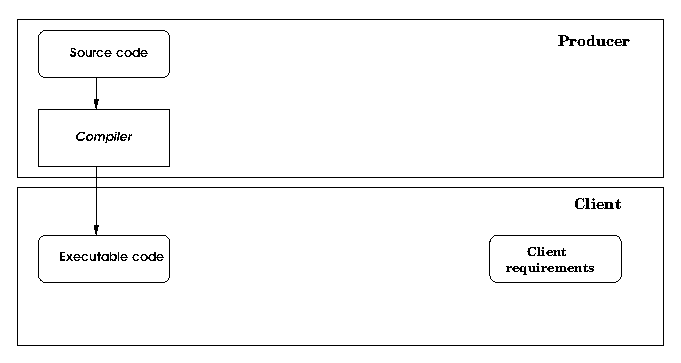
\epsfig{file=figs/mobileCode.eps}
%\caption{Mobile code}
\end{center}
%\end{frameit}
\end{figure} 
}


%2.2
\frame[shrink,containsverbatim]{
 \frametitle{What are the different approaches}
 \begin{itemize}
   \item type based verification  
        \begin{itemize}
               \item e.g. the bytecode verifier in the Java Virtual Machine (JVM) 
               \item only guarantees that the verified code does not corrupt  the JVM 
         \end{itemize}
   \item dynamic checks 
        \begin{itemize} 
                \item e.g. the sandbox mechanism in Java  % is this stack inspection mechanism
		\item runtime overhead  
        \end{itemize}
    \item program logic  verification 
         \begin{itemize} 
                \item e.g. verification tools like esc/java, Jack, Jive, Loop tool \ldots
                \item powerful, may verify for complex functional and security properties
	        \item however \ldots 
	 \end{itemize}
 \end{itemize}
}

%2.1
\frame[shrink]{
\frametitle{Source verification architecture}
\begin{figure} 
\begin{center}
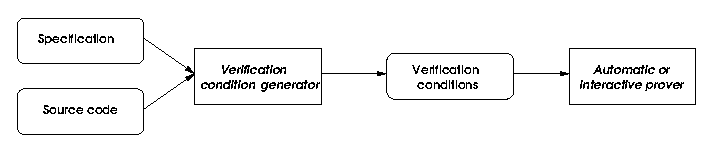
\epsfig{file=figs/sourceVerification.eps} % , width=5in, height=3in }
%\caption{Source verification architecture}
\end{center}
\end{figure}
}





%2.3
\frame[shrink]{
\frametitle{Mobile code verification}
\begin{figure}[hc]
\begin{center}
%
\includegraphics{bc.eps}
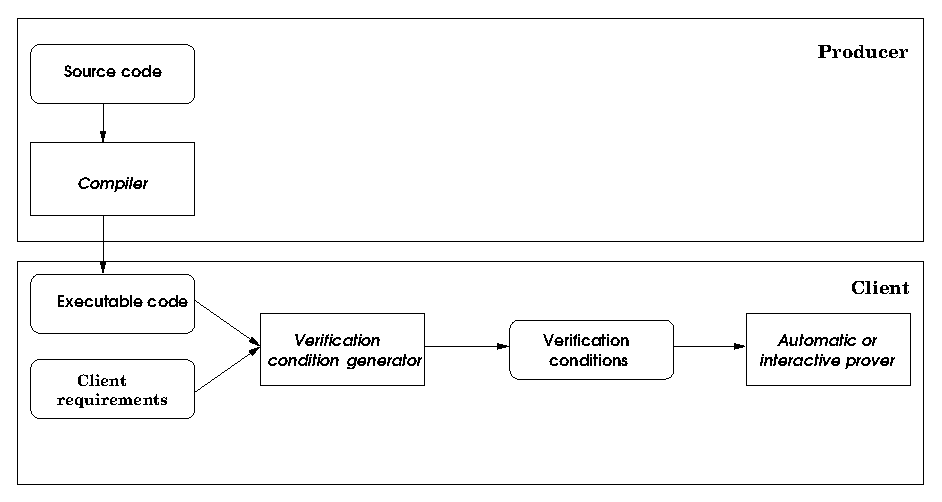
\epsfig{file=figs/mobileCodeVerif.eps}
%\caption{\sc Mobile code verification}
%\label{intro:mobileVerif}
\end{center}
\end{figure}
}



%2.4
\frame[shrink]{
\frametitle{Proof carrying code architecture for mobile code}
\begin{figure}[hc]
\begin{center}
%
\includegraphics{bc.eps}
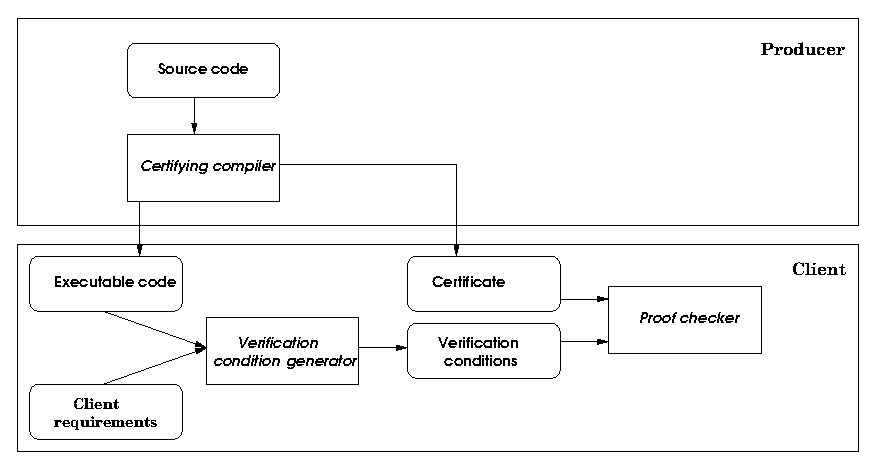
\epsfig{file=figs/PCC.eps}
%\caption{\sc Mobile code verification}
%\label{intro:mobileVerif}
\end{center}
\end{figure}
}

%.2.5
\frame[shrink]{
\frametitle{Proof preserving compilation for mobile code}
\begin{figure}[hc]
\begin{center}
%
\includegraphics{bc.eps}
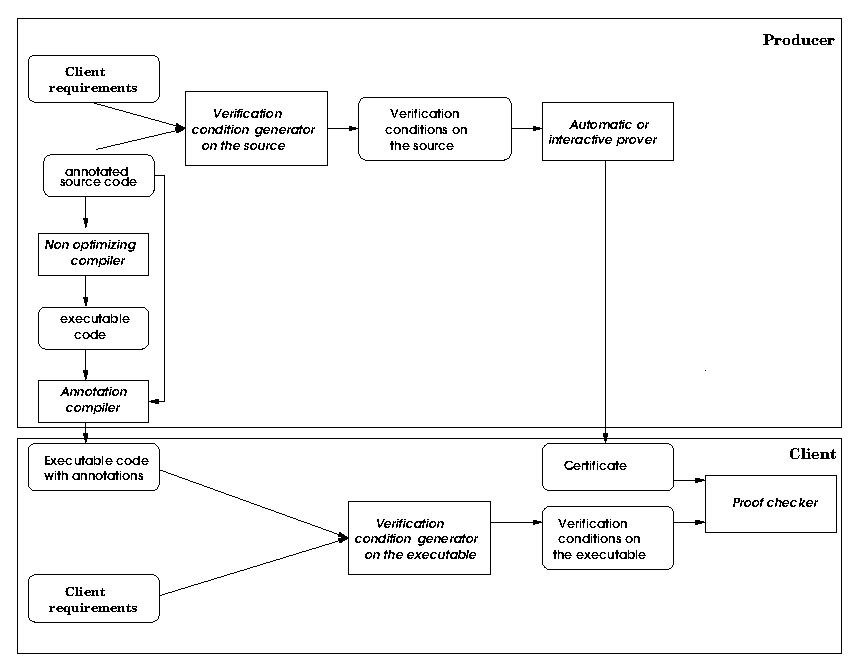
\epsfig{file=figs/PPO.eps}
%\caption{\sc Mobile code verification}
%\label{intro:mobileVerif}
\end{center}
\end{figure}
}

\frame[shrink]{
\frametitle{Approach}
\begin{figure}[hc]
\begin{center}
\begin{itemize} 
       \item Bytecode Modeling Language (BML)  
       \item a compiler from source annotations to bytecode annotations
       \item verification condition generator for bytecode  
       \item relation between verification conditions on source and non optimized bytecode    
             
\end{itemize}
\end{center}
\end{figure}
}

%==================================================================================
%==========================BML=====================================================
%==================================================================================

\section{Bytecode Modeling Language}


%==================================================================================
%=================================VERIFICATION CONDITION GENERATOR=================
%==================================================================================


% verification condition generator for bytecode
\section{Verification condition generator for Java bytecode}
\subsection{Overview of program verification}
\frame[shrink]{
\frametitle{What is the problem of program verification ?}
\begin{block}{What do we verify?} 
 Program w.r.t.   program specification consisting of 
   \begin{itemize} 
       \item precondition %, which states the property that must have initial states    
       \item postcondition % which states the property that must hold when the method terminates
    \end{itemize}
\end{block}
\pause
\begin{block}{Partial correctness condition}
  A program \program~ respects a precondition \textit{Pre} and a 
 postcondition \textit{Post}  if for every initial state of  \program~ which satisfies \textit{Pre}
 if \program~ terminates, then it terminates  in a state which  satisfies \textit{Post}
\end{block}
}


  % why a verification condition generator
  % comparison with another possibilities for doing verification 
\frame{\frametitle{Comparison between different approaches}
 \begin{itemize}
       \item perform the verification directly over the operational semantics
               \pause  \begin{itemize} 
                             \item  needs intensive user interaction
			\end{itemize}
                       \pause	
       \item use a Hoare style logic \pause 
                \begin{itemize} 
                        \item better than the previous approach, however still hard to automize 	
                \end{itemize}      
			  \pause	
       \item verification condition generator
                 \pause 
                \begin{itemize} 
                        \item a completely automatic procedure  	     
               \end{itemize}
     \end{itemize}
}
 




% how all these schemes are realised - the use of specification language
\frame{\frametitle{Components of the verification procedure}
 \begin{itemize}
       \item specification of the application which expresses the intended behavior of the program
                       
       \item an algorithm for generating logical formulas whose validity implies the program correctness
                      
       \item a procedure for checking the validity of the verification conditions, automatic decision procedures, 
             interactive theorem provers
  \end{itemize}
}


 \section{Relation between bytecode and source verification conditions}


 \section{Applications}
 \subsection{Java-to-Native Compilation}


\frame[shrink]{\frametitle{Java-to-Native Compilation}
Compiling Java bytecode into native code brings runtime advantages:
\begin{itemize}
    \item Faster execution
    \item Especially beneficial for restrained systems with non-sophisticated JVMs
\end{itemize}
But Java-to-Native compilation also comes with drawbacks:
\begin{itemize}
    \item Native code is typically 3 to 4 times bigger than bytecode,
\end{itemize}
}


 \frame[fragile,shrink]{\frametitle{Why is Native Code so Huge? }

The \emph{idiv} bytecode throws an \texttt{ArithmeticException} if the divisor is equal to zero:

%\begin{columns}
%\begin{column}{3.1cm}
\begin{lstlisting}[language=JVMIS]
iload i
iload j
idiv
ireturn
\end{lstlisting}
%\end{column}
%\begin{column}{3.1cm}
}



 \section{Future work}
     \subsection{Results}

     \subsection{Future directions}
 
\end{document}
